\documentclass{elsart}
\usepackage{natbib}
\usepackage{epsfig}
\usepackage{amssymb}

\begin{document}
\runauthor{Oswald et.al.}
\begin{frontmatter}
\title{Various methods of calibration of the STEREO/WAVES antennas}
\author[iwf]{T.H. Oswald}
\author[iwf]{W. Macher}
\author[iwf]{H.O. Rucker}
\author[iowa]{G. Fischer}
\author[iwf]{U. Taubenschuss}
\author[med]{J.L. Bougeret}
\author[med]{A. Lecacheux}
\author[green]{M.L. Kaiser}
\author[min]{K.Goetz}


\address[iwf]{Space Research Institute, Austrian Academy of Sciences, Graz, Austria}
\address[iowa]{University of Iowa, Iowa City, IA, USA}
\address[med]{Observatoire de Paris-Meudon, France}
\address[green]{NASA/GSFC, Greenbelt, MD, USA}
\address[min]{University of Minnesota, Minneapolis, MN, USA}

\begin{abstract}
On October $25^{th}$, 2006, NASA�s two STEREO spacecraft were launched which are designed to increase our knowledge of the physics of the solar system. On board they carry a sophisticated radio experiment, called S/WAVES. The key technology, used by S/WAVES is the direction finding capability in addition to the use of two spacecraft which makes it possible to triangulate radio sources. Direction finding requires the reception properties of the antennas to be known very accurately. We applied several different methods to calibrate the S/WAVES antennas. In this paper the methods are described and compared and the results are presented and discussed with respect to advantages and disadvantages of the different methods.
\end{abstract}

\begin{keyword}
STEREO, S/WAVES, antennas, antenna calibration, solar radio waves
\end{keyword}
\end{frontmatter}

\parindent=0.5 cm

\section{Introduction}
On October $25^{th}$, 2006, NASA launched the two STEREO spacecraft with a radio experiment on board, called STEREO-WAVES (S/WAVES), which is designed to observe solar radio emissions by using direction finding capabilities. The S/WAVES experiment is designed to track solar and interplanetary radio bursts and trace the generation and evolution of radio disturbances from the Sun to the Earth orbit and beyond. Each spacecraft has three nearly orthogonal antennas, capable of receiving electromagnetic waves in several frequency ranges. The main operation range of the receivers is between 10kHz and 16MHz. With this configuration, it is possible to perform direction finding at the lower end of the frequency range to determine the direction of incidence and the polarization of the received radiation. When both spacecraft receive radiation from the same source, the actual location of the source can be pinpointed by the method of triangulation.

For the correct interpretation of the data it is of vital
importance to know the antenna properties with great accuracy. The magnitude and direction of the effective length vectors are parameters of the usual direction finding methods [\cite{cecconi05}].
%
We performed the antenna calibration using two numerical and one
experimental method. Each method has its own merits. The results are
very consistent and are presented in this work.


\subsection{The spacecraft and the S/WAVES experiment}
The STEREO/WAVES experiment works with three mutually orthogonal stacer
monopole antennas. They are connected to several receivers which can operate in the following modi:

\begin{itemize}
    \item FFR   fixed frequency receiver\\
\item HFR   high frequency receiver\\
\item LFR   low frequency receiver\\
\item TDS   time domain sampler\\
\item LWS   Langmuir wave statistics\\
\item LRS   low rate science\\
\end{itemize}


In this paper we will be dealing with the HFR and with band B and C of
the LFR. The HFR operates in a range from 125 kHz to 16.025 MHz. The HFR provides 12 bit data in contrast to the 8 bit data of older receivers like the CASSINI/RPWS
receiver, and will provide all auto- and cross-correlation
parameters. Two direction finding modes are planned, one of which
uses the antennas as dipoles, like RPWS did. The other DF mode uses
the antennas as monopoles. Each sweep will take approximately 15
seconds.

The LFR comprises 3 frequency bands, A, B and C. The ranges are
%
\begin{itemize}
    \item A: 2.5-10 kHz\\
\item B: 10-40 kHz\\
\item C: 40-160 kHz\\
\end{itemize}

Bands B and C provide auto- and cross-correlation parameters and can be used
for DF. The data produced by the LFR also has an accuracy of 12 bits.
Hence, the frequency range of interest in this paper is between 10kHz
and 16MHz.


The FFR operates at one of two frequencies at approximately 30MHz and 32MHz.
To deal with the calculations of antenna properties at this
frequency requires totaly different considerations, therefore the
calculation of the antennas for use in combination with the FFR will
be presented in another article.



\subsection{The effective length vector as representation of the
transmitting and receiving antenna}
A highly useful concept which will be used extensively in this article is the effective length
vector $\textbf{h}_e$. It can be defined as a vector such that the equation


\begin{equation}\label{antenna_equation}
 V=\textbf{h}_e \cdot \textbf{E}
 \end{equation}

is satisfied for a received monochromatic electromagnetic wave. V is the
voltage induced at the feed and $\mathbf{E}$ the electric field of the incident monochromatic wave. The effective length vector is in general a complex quantity and depends on the direction and frequency of the incident wave.

At the moment we are assuming vacuum as surrounding medium, which means that the reciprocity theorem is applicable. Hence the concepts of a receiving and transmitting antenna is equivalent in terms of certain antenna properties. Dealing with a transmitting antenna results in an easier method when doing the calculations. Hence, we determine the parameters which describe the behavior of a transmitting antenna which is driven by a unit voltage at the feed and deduce from them the properties of the same antenna in a receiving condition.

Due to the fact that the skin of a spacecraft is conducting, it is coupled electromagnetically to the monopole and has to be considered as part of the antenna system. So the receiving properties depend on the shape and construction of the spacecraft. The effective length vector comprises much information of this shape. The usefulness of the concept of the effective length vector can be understood by realizing that the complicated shape of the spacecraft hull can be condensed into a single vector representing the antenna properties. The effective length vector can be calculated by the following integral [\cite{macher_dipl,Sinclair,CollinZucker}].

\begin{equation}\label{heff}
\textbf{h}_e=\frac{1}{I}\int \mathbf{J}(\mathbf{r}')e^{\imath
\mathbf{k} \cdot \mathbf{r}'} dV'
\end{equation}

$\mathbf{J}(\mathbf{r}')$ is the current density induced in the antenna when driven with the current I at transmission, while $-\mathbf{k}$ is the wave vector received in reception mode. The dependencies on frequency and direction can safely be neglected at low frequencies, where the effective length vector can be regarded as real and constant. This range is called the quasistatic range. In this frequency range, most known direction finding techniques work with satisfying accuracy. It is of vital importance to know the upper boundary of this range. For the STEREO/WAVES antennas the boundary is estimated to be approximately 2 MHz as described later.

\begin{figure}
\begin{center}
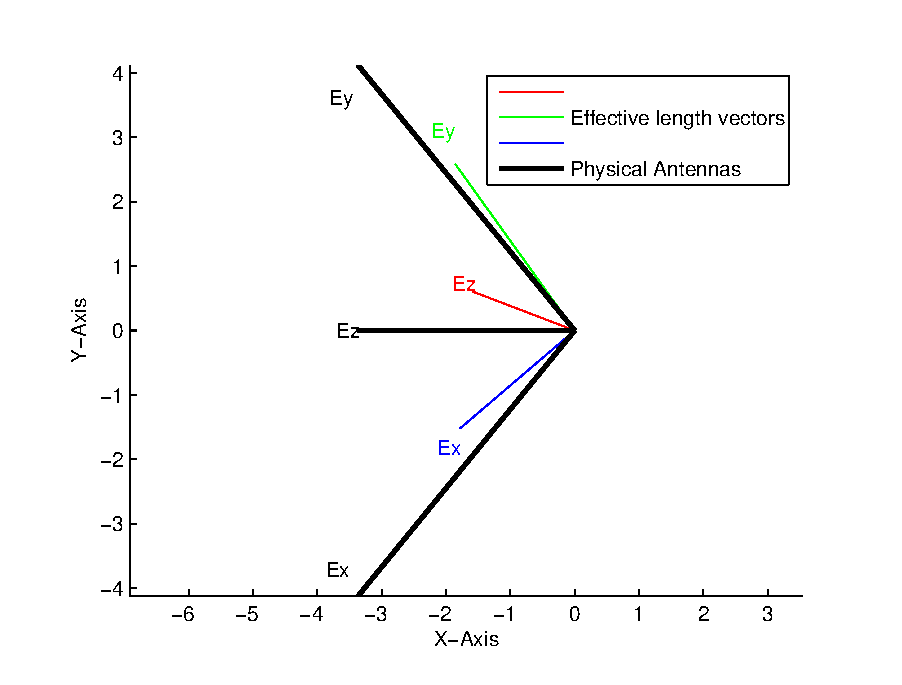
\includegraphics[width=12cm]{PaperPics/fig(2).eps}
\end{center}
\caption{\label{comparison}Comparison of geometric antennas and effective length vectors}
\end{figure}

The effective length vectors often deviate considerably from the geometric antennas. Figure \ref{comparison} shows the geometric antennas of the STEREO spacecraft in black, while the effective length vectors are shown in color. For this calculation a frequency of 300kHz was used which is well within the quasistatic range.


At high frequencies, where the wavelength of the incident wave can not be regarded as large in relation to the spacecraft dimensions, the effective length vector depends on frequency and direction of the radiation  (see eq. (\ref{heff})) and its imaginary part becomes significant. Special care has to be taken when the effective length vectors are used in this range.

\section{The numerical method}
The calculation  has to be done in two steps. First the current distribution is computed by using the Method of Moments (MOM). Then, in a second step the effective length vectors and other interesting parameters describing the antenna behavior are calculated.

\begin{figure}
\begin{center}
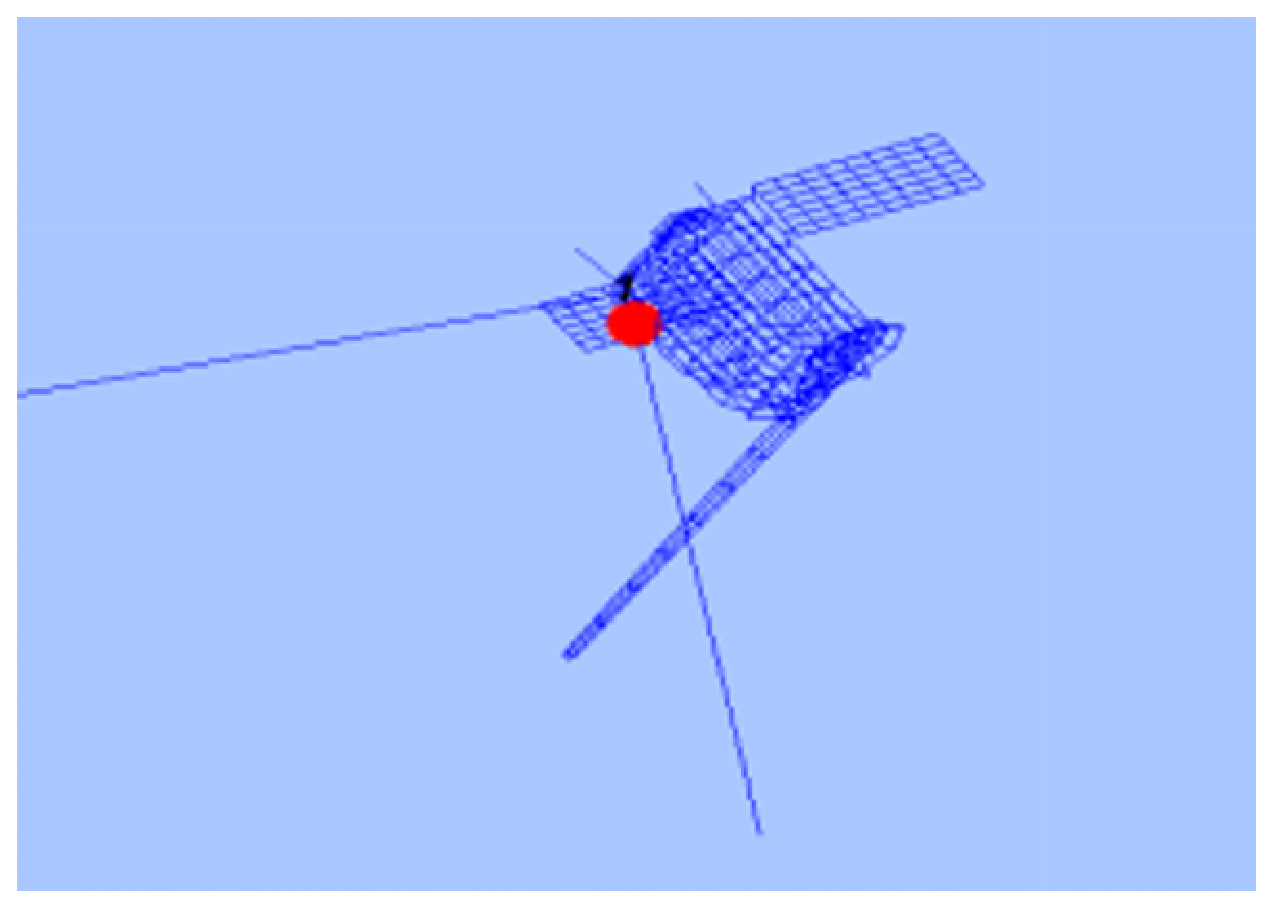
\includegraphics[width=12cm]{PaperPics/fig(3).eps}
\end{center}
\caption{\label{wiregrid}The wire-grid model}
\end{figure}


\subsection{Calculation of the current distribution}
The calculation of the current distribution on the surface of the spacecraft was done by using a modified version of the Antenna Scatterers Analysis Program (ASAP), which is a very popular open source program based on a well proved electromagnetic code and CONCEPT II, a proprietary software written at the University of Hamburg-Harburg.

The current distribution is calculated by solving the appropriate integral equation, which is the electric field integral equation (EFIE) in case of CONCEPT and the reaction integral equation (RIE) in case of ASAP.

For the calculation of the surface currents with ASAP or CONCEPT the spacecraft is modeled as a wire-grid  (Figure \ref{wiregrid}). The antennas are excited at their feed points with an electromotive force of 1V. One of the feeds is marked by the red dot in Figure \ref{wiregrid}. Instead of the surface currents, the currents along the wires are calculated, so the surface integral (\ref{heff}) is transformed into a sum of scalar line integrals where each line integral has to be solved along a wire segment. Both programs are only dealing with currents parallel to the wires, transverse currents are neglected.

ASAP uses a piecewise-sinusoidal expansion to represent the currents along the wires while CONCEPT uses triangular functions. In the quasistatic case where the wavelength is much longer than the wire segments those two representations are equivalent, at higher frequencies one might prefer the sinusoidal expansion.

The integral equation has to be solved in conjunction with the boundary conditions. Both programs use the MOM [\cite{harrington}] to transform the integral equation into a matrix equation of the form

\begin{equation}\label{matrix_eq}
    \mathbf{ZI}=\mathbf{V}
\end{equation}

This equation can be solved for \textbf{I} by methods of linear algebra. \textbf{V} is a vector which holds the excitation voltages. In the case of the transmitting antenna almost all elements are zero. Only the element which represents the driven feed holds a unit voltage. \textbf{Z} is the impedance matrix which holds the impedances of the wire segments. The diagonal elements represent the self impedances of each segment, the off-diagonal elements hold the mutual impedances between the different segments. Vector \textbf{I} is the unknown quantity and holds the coefficients of the base functions. In case of ASAP, pairs of segments are used to form small dipoles. Hence in this solution method \textbf{Z} represents the impedance matrix of these dipoles.

In the frequency range where the two programs are used here the two methods are equally valid, so the results must be consistent.  This can be used as a test for the validity of the method and the model.

\subsection{Calculations of the antenna parameters}
Based on the surface currents \textbf{J}, the effective length vectors, the fields, the radiation pattern and the impedances can be computed. This was done by using Matlab functions. The main advantage of this numerical method is
flexibility with regard to the representation of spacecraft parts, which can easily be altered to test their influence on antenna properties. The calculation was done for open feeds and for loaded feeds where the total base capacitance  (receiver, cable, and antenna mounting) was estimated to be 70 pF.

The input impedance can be computed by dividing the voltage at the feed by the current.

The next step is the calculation of the effective length vectors by applying equation (\ref{heff}).Using the effective length vector, the response of an antenna to an incident wave can be calculated by means of equation (\ref{antenna_equation}).

The relation between the vector potential $\mathbf{A}(\mathbf{r})$ in the far field at position $\mathbf{r}$ and the effective length vector is

\begin{equation}
  \mathbf{A}(\mathbf{r}) = \frac{\mu_0 I \textbf{h}_e}{4 \pi r}e^{-\imath k r}
\end{equation}

with $\mu_0$ as the permeability of free space. On base of the vector potential all other fields of the transmitting
antenna can be computed with the standard equations. Details of the derivations of the equations can be found in [\cite{macher_dipl}].


Finally the effective length vector can be used to compute the gain of the antenna

\begin{equation}
    G(\mathbf{k}) \propto \left| \frac{\mathbf{k}}{k}\times \mathbf{h}_e \right|^2
\end{equation}

\section{The experimental method: Rheometry}

\begin{figure}
\begin{center}
\includegraphics[width=12cm]{PaperPics/fig(4).eps}
\end{center}
\caption{\label{rheomodel}The rheometry model of the STEREO spacecraft}
\end{figure}


The rheometry measurements allow to determine the effective axes and lengths of the antennas for the quasi-static frequency range. A gold plated model of the antennas-spacecraft system has to be built (Figure \ref{rheomodel}). This model is immersed in an electrolytic tank (in our case tap water serves as electrolyte). Metal plates are attached to two opposite sides of the tank to form a large capacitor. A signal generator is connected to the plates to sustain a homogeneous electric field in the tank. The voltages at the model antennas are measured as a function of the model orientation. For that purpose the model can be rotated around a vertical axis, and different suspensions of the model at this axis are used. So the induced voltages for a variety of orientations of the model with regard to the electric field direction are recorded, from which the effective length vectors can be inferred.

The reason, why an electrolytic fluid is needed, is the extremely high impedance of the model antennas in air, which exceeds the input impedance of the voltmeter. So connecting the voltmeter to an antenna terminal would bias the measured voltages. This problem can be overcome by immersing the model in an appropriate electrolyte, thereby additionally reducing the influence of stray fields. To prevent polarization effects an alternating electric field with an appropriate frequency of about 1kHz must be used. Further details can be found in [\cite{rheometry} and \cite{macher07}], where a theoretical treatment as well as practical aspects of the measurement principle are given.

The results of rheometry represent the asymptotic behavior of the reception properties for the transition to very low frequencies, where many numerical codes get inapplicable due to bad condition of the underlying numerical inversion. A further advantage of this method is that very fine details of the spacecraft body can be modeled, whereas numerical methods soon reach their limit when small parts near the antenna feed zone have to be modeled.

\section{Other methods}
The anechoic chamber is also often used for the antenna calibration of spacecraft. As in rheometry a small scale model of the spacecraft is used for the measurement. It is illuminated by coherent electromagnetic radiation of various wavelengths. During the measurement process the response of the antennas due to the incoming radiation is measured as a function of the orientation of the model.

The advantage of this method in comparison with rheometry is the possibility to use different wavelengths, therefore deducing the behavior in different frequency regions above the quasistatic limit. Also due to the setup of the measurement, it is free of the disturbing influence of the environment.


\begin{figure}
\begin{center}
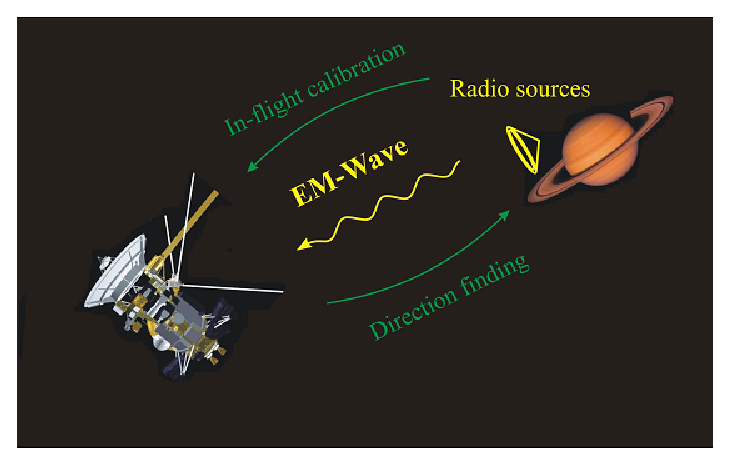
\includegraphics[width=12cm]{PaperPics/fig(5).eps}
\end{center}
\caption{\label{inflight}In-flight calibration of the Cassini/RPWS antennas as opposed to direction finding.}
\end{figure}

In-flight calibration is a technique to determine the properties of an antenna when the spacecraft is spaceborne. A source of known position and magnitude which might be natural or manmade, is used. Ideally the response of the antennas in different receiver modes is measured in combination with different spacecraft orientation. Such calibrations will be performed for the S/WAVES antennas when STEREO has collected enough data. Special maneuvers have been provided to support this activity (Figure \ref{inflight}). Direction finding and in-flight calibration can be seen as reciprocal procedures. In-flight calibration is the procedure of determining the effective length vectors by using a known source, while direction finding yields information about the radio source, requiring the knowledge of the effective length vectors.

\section{The results of the determination of the effective length vectors of the S/WAVES antennas}
\subsection{Introduction}
Numerical calculations, using ASAP and CONCEPT II, as well as rheometry measurements were performed to determine the characteristics of the three antennas of the S/WAVES experiment. Similar calculations were done in the past for the Cassini spacecraft [\cite{cassini,cassini2,vogl_04}] as well as for Mars Express [\cite{marsis,marsis2}] and other spacecraft. A summary can be found in [\cite{ruckerundi05}].

\subsection{The characteristics of the spacecraft and the model}

\begin{figure}
\begin{center}
\includegraphics[width=12cm]{PaperPics/fig(6).eps}
\end{center}
\caption{\label{stereo1}Illustration of one STEREO spacecraft and its coordinate system�}
\end{figure}

One characteristic of the STEREO spacecraft is a certain degree of asymmetry (Figure \ref{stereo1}). In contrast to many other spacecraft, the solar panels are positioned at asymmetrical positions with regard to the spacecraft hull. Additionally, the spacecraft comprises an about 6 meters long boom, and a turnable high gain antenna. These prominent features have an influence on the antenna characteristics. The boom is divided into 4 sections with different diameters and has great influence upon the effective length vectors of the antennas.


The spacecraft fixed reference frame is defined in such a way that the positive x-axis points to the Sun most of the time. The antennas are mounted on the side of the hull which points to the negative x-axis, so they remain out of view of the sunward looking instruments on the spacecraft. The solar panels are parallel to the positive and negative y-axis and the z-axis is defined to complete the right handed cartesian frame (Figure \ref{stereo1}).

For the description of the direction of the antennas we use spherical coordinates which have the positive x-axis as polar axis. The angle $\zeta$ is the angle between the positive x-axis and the antenna, and $\xi$ is the azimuthal angle around the x-axis, where antenna $E_z$ has $\xi=0$.

The direction of the boom defines the negative x-axis. There are 3 orthogonal monopole antennas, which are called $E_x$, $E_y$, and $E_z$, each 6 meters long. They are directed about $125.26^\circ$ from the x-axis and the difference in azimuth is $120^\circ$. The azimuth of antenna $E_z$ as well as the negative z-axis define the azimuth of $0^\circ$, which is increasing counter-clockwise when viewed from the positive x-axis. It is expected, that the boom has an effect to push the 3 electrical antennas away from the boom's position. This effect is increased by the high gain antenna, which is located near the boom. The panels are expected to push the effective length vectors towards the negative x-axis.

The two spacecraft A and B are almost identical, apart from some small differences of their instrumentation. The only difference which can be modeled within the limitations of the algorithm is the second ring, mounted on the hull of spacecraft B on the positive x-side, and not existent on spacecraft A. The rheometry model can be constructed with much more detail, so more differences between the two spacecraft can be taken into account at the rheometry measurements.

The wire-grid model of the STEREO spacecraft consists of the following parts:

\begin{enumerate}
\item The hull
\item 2 solar panels
\item The high gain antenna
\item Three 6 meter long antennas
\item A 6 meter long boom
\item A ring mounted on the hull of spacecraft A, two rings on spacecraft B\\
\end{enumerate}

\begin{figure}
\begin{center}
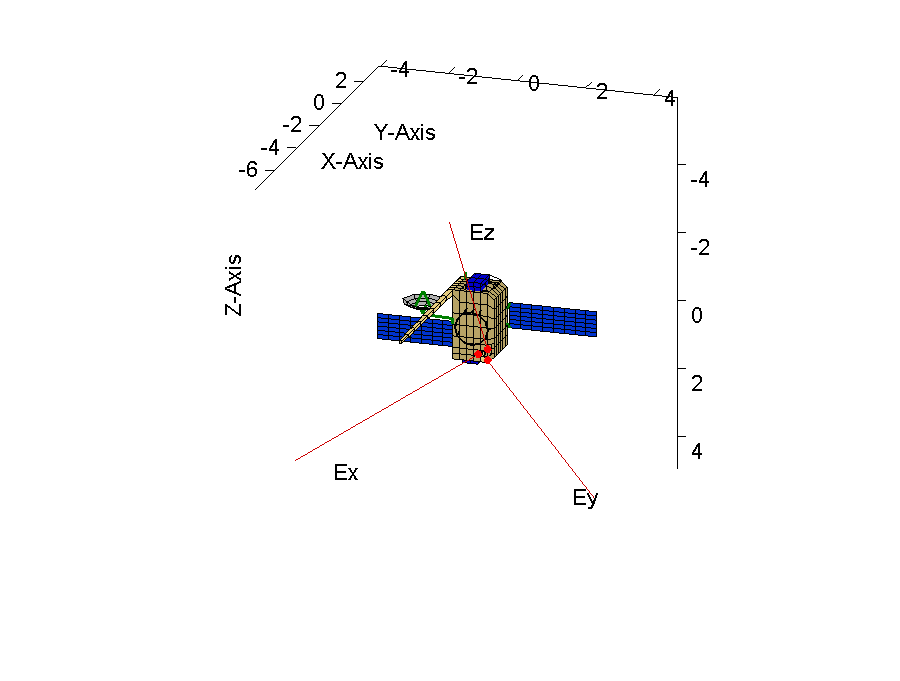
\includegraphics[width=12cm]{PaperPics/fig(7).eps}
\end{center}
\caption{\label{fig_stereo_model}The STEREO wire-grid model}
\end{figure}

Size and position of the parts were measured from the relevant construction plans. The boom is modeled as prism with rectangular base. Figure \ref{fig_stereo_model} shows the model from an oblique view.

\subsection{The determination of the effective length vectors at the quasistatic limit}
 For the analysis of the properties at the quasistatic limit we chose the results at 300kHz. Below this frequency there might be the possibility of numerical artifacts, while above this frequency the effects of the shorter wavelength in relation to the spacecraft dimensions might influence the results.

Also rheometry measurements were performed. A correction for the real antenna diameter had to be applied for the rheometry results and the results which were obtained by using ASAP. The CONCEPT II software allows different diameters of individual segments, so we were able to take the antenna diameters into account directly.

\begin{table}[htbp]
\caption{STEREO A, physical and effective antennas with open feeds determined by use of ASAP and CONCEPT II at 300kHz, and rheometry} \label{tab_heff1}
\begin{tabular*}{\hsize}{llllll}
\hline
 &  & ASAP & CONCEPT  & rheo & physical \\
\hline
& l/m & 3.03 & 3.02& 2.89 & 6.00\\
  $E_x$ & $\zeta$/$^\circ$ & 126.0 & 125.4 & 126.2  & 125.3\\
& $\xi$/$^\circ$ & -141.4 & -141.3  & -140.7& -120.0 \\
\hline
& l/m & 3.82 & 3.81 & 3.84 & 6.00\\
  $E_y$ & $\zeta$/$^\circ$ & 119.1 & 118.6 & 118.7& 125.3\\
& $\xi$/$^\circ$ & 129.1 & 129.0 & 127.9 & 120.0\\
\hline
& l/m & 2.31 & 2.30 & 2.36& 6.00 \\
  $E_z$ & $\zeta$/$^\circ$ & 133.7& 133.3 &132.2 & 125.3\\
& $\xi$/$^\circ$ & 21.4 & 21.4 & 21.6& 0.0\\
\hline
\end{tabular*}
\end{table}


\begin{table}
\caption{STEREO A, physical and effective antennas with loaded feeds determined by use of ASAP and CONCEPT II at 300kHz, and rheometry}
\label{tab_heff3}
\begin{tabular*}{\hsize}{llllll}
\hline
&  & ASAP & CONCEPT  & rheo & physical \\
\hline
& l/m & 1.36 & 1.35 &1.34 & 6.00\\
  $E_x$ & $\zeta$/$^\circ$ & 120.2 & 119.9 &121.3 & 125.3\\
& $\xi$/$^\circ$ & -135.8 & -135.3 &-135.4 & -120.0 \\
\hline
& l/m & 1.66 & 1.64 &1.69 & 6.00\\
  $E_y$ & $\zeta$/$^\circ$ & 115.2  &114.4 &115.1 & 125.3\\
& $\xi$/$^\circ$ & 127.5 & 127.3 &126.8 & 120.0\\
\hline
& l/m & 1.10 & 1.09  &1.13 & 6.00 \\
  $E_z$ & $\zeta$/$^\circ$ & 125.7& 124.7 &125.3 & 125.3\\
& $\xi$/$^\circ$ & 15.9 & 15.5 &16.4 & 0.0\\
\hline
\end{tabular*}
\end{table}



The result of the calculations can be seen in Table \ref{tab_heff1} for open feeds and in Table \ref{tab_heff3} for loaded antennas with base capacitances of 70pF. This value for the base capacitances was chosen on basis of new measurements performed at the Space Science Laboratory in Berkley, CA. Due to improved measurement procedures, this value is more realistic, than the old value of 90pF, which was used in [\cite{macher07}]. The change of the base capacitances results in a small increase of the lengths of the effective length vectors, while the directions are hardly affected. The frequency is 300kHz which is well in the quasistatic limit. For comparison, the lengths and orientations of the physical antennas are also added.

The quasistatic results are in full concurrence with our expectations. The magnitudes of the effective length vectors for open feeds are about half the length of the physical antennas, as expected by theory for short monopoles. In this context, short means short in relation to the wavelength. The influence of the capacitances on the effective length vectors is quite substantial. Furthermore, it can clearly be seen that the solar panels push the electric antennas towards the negative x-axis with a counteracting influence of the boom. The results of the numerical and experimental determination are very consistent.

\subsection{Variation of the properties with frequency and direction}
The wire-grid currents at frequencies from 100 kHz to 34 MHz were calculated by using ASAP and CONCEPT II in turn. The frequency spacing was 100 kHz. Using this data, the impedances, admittances and effective length vectors were computed with MATLAB routines. The direction of the incident wave was taken to be the positive x-axis, simulating radiation from the Sun.


\begin{figure}
\begin{center}
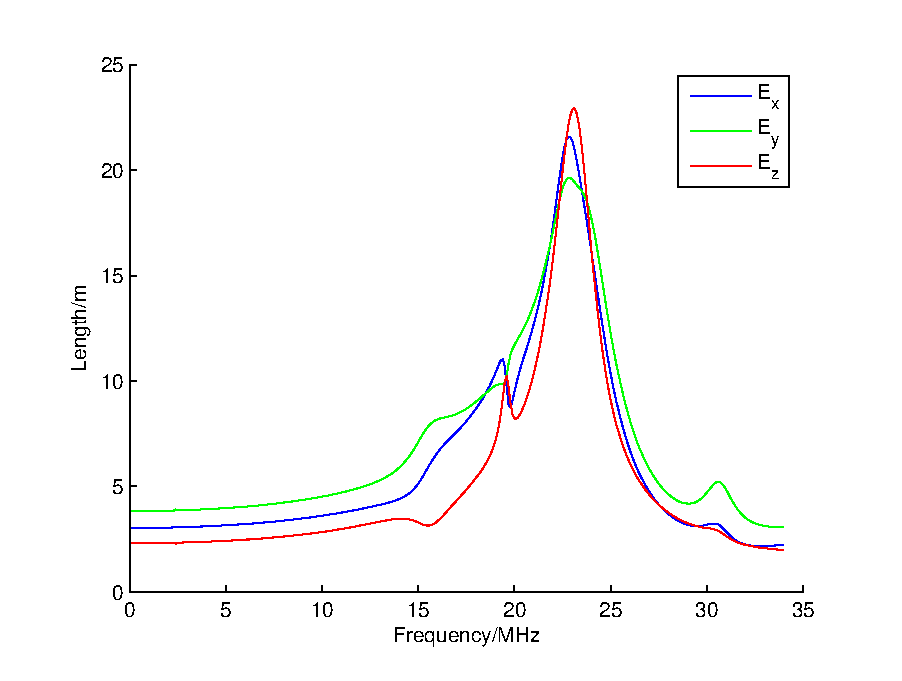
\includegraphics[width=12cm]{PaperPics/fig(8).eps}
\end{center}
\caption{\label{fig_hefflength_abs}Magnitude of the effective length vector as a function of frequency}
\end{figure}


Figure \ref{fig_hefflength_abs} shows the magnitude of the effective length vector as a function of frequency. The direction of incidence was taken to be the x axis which corresponds to the direction of the Sun. Between 20 and 25MHz there is a resonance which occurs when the distance between the antenna tip and the most distant part of the spacecraft body, which is the remote corner of the opposite solar panel. This corresponds to the second antenna resonance and the lowest maximum of its radiation resistance (the real part of the antenna impedance, see Figure \ref{fig_imp_open}). When the antenna resonates, its response to the radiation is very strong which corresponds to a large effective length vector.

\begin{figure}
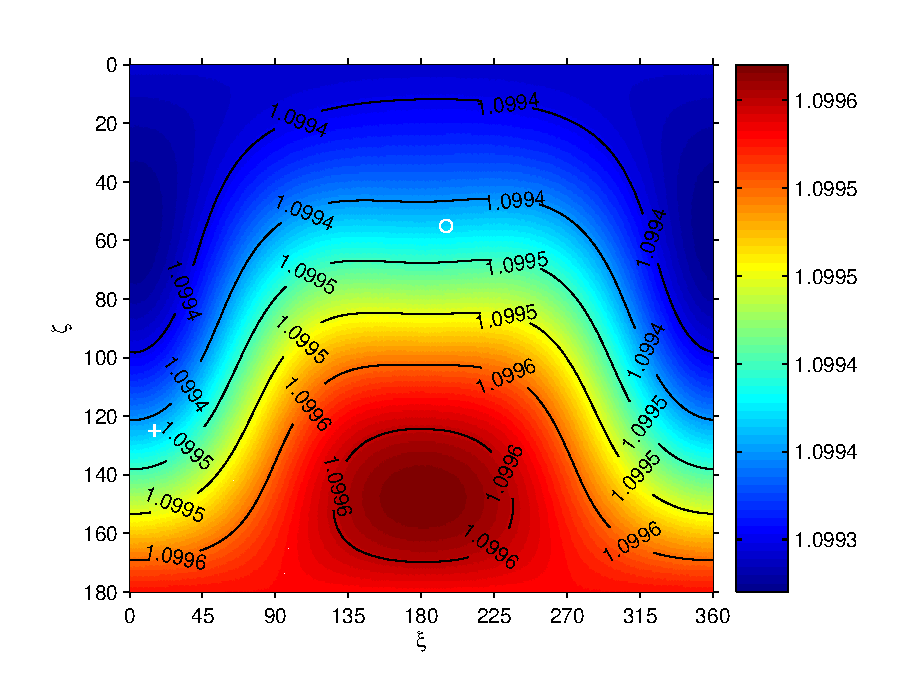
\includegraphics[width=7.6cm]{PaperPics/fig(9).eps}
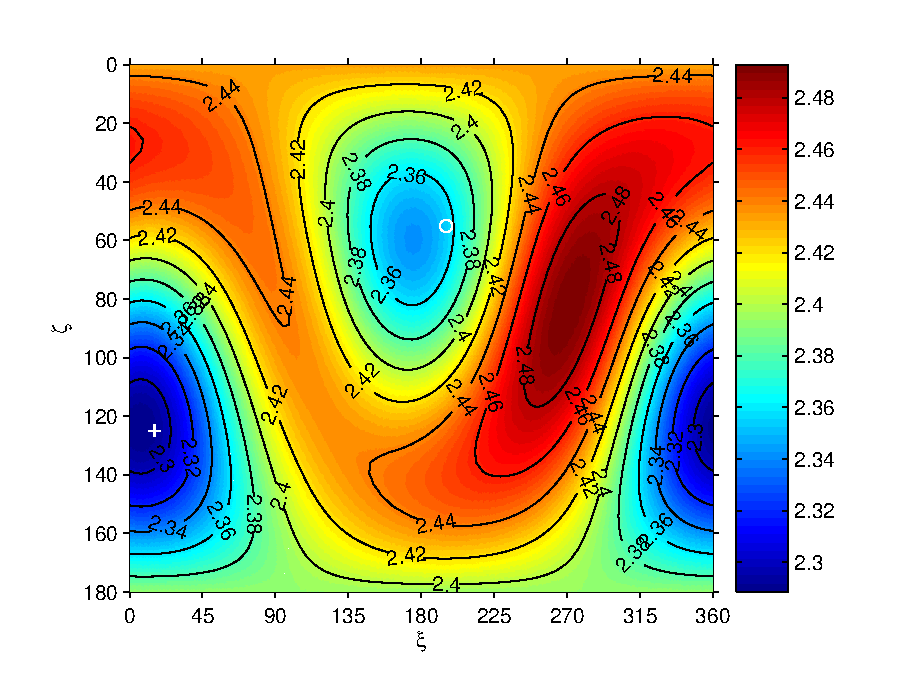
\includegraphics[width=7.6cm]{PaperPics/fig(10).eps}
\caption{\label{fig_var_dir}Magnitude of the effective length vector of antenna $E_z$ as a function of direction of incidence ($\zeta$ and $\xi$ in radians) at 300kHz (left) and 10MHz (right). Note the different scaling of the color bars.}
\end{figure}

Figure \ref{fig_var_dir} shows the magnitude of the effective length vector of antenna $E_z$ as a function of the direction of incidence at 300kHz and 10MHz respectively, using open feeds. The variability at 300kHz is negligible which is not true at 10MHz. This has to be taken into account when data at high frequencies are analyzed.

Direction finding can be performed, yielding useful results, with the known methods when the directions of the electric antennas are known with an accuracy of about 2 degrees. Detailed analysis of antenna properties of the S/WAVES antennas indicate an upper limit of not more than 2MHz. Above this limit the effective length vectors deviate significantly from the quasistatic case, so direction finding can only be performed with limited accuracy or with methods which take the dependance on frequency and direction into account. Figure \ref{fig_var_dir} suggests that even at higher frequencies and in the region near the resonance frequency, the effective length vectors behave moderately when the direction of incidence is changed. The same is true for frequency variations.

\subsection{Variation of the effective length vectors with different HGA orientations}
The high gain antenna (HGA) on the STEREO spacecraft is mounted turnable which is illustrated in Figure \ref{fig_hga}.  The effect of the HGA orientation on the effective length vectors was investigated.

\begin{figure}
\begin{center}
\includegraphics[width=12cm]{PaperPics/fig(11).eps}
\end{center}
\caption{\label{fig_hga}The turnable high gain antenna}
\end{figure}

Analysis of the influence of the orientation of the HGA upon the effective length vectors has shown that the resulting deviation is negligible. As an example, Figure \ref{fig_var_HGA} shows the magnitude of the effective length vectors as function of the angle of the HGA with open feeds at 300kHz and 10MHz, respectively.

\begin{figure}
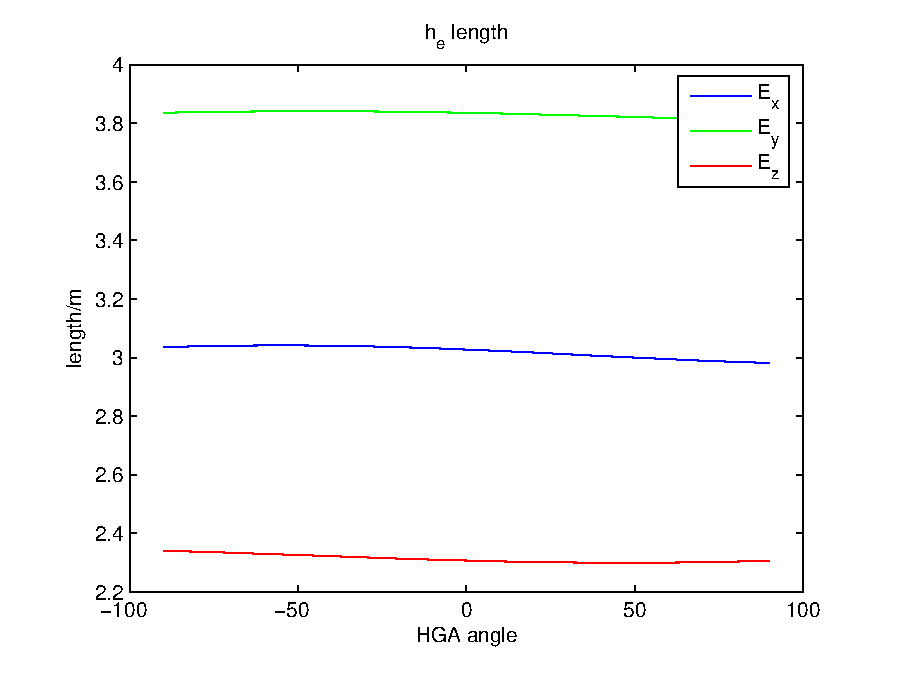
\includegraphics[width=7.6cm]{PaperPics/fig(12).eps}
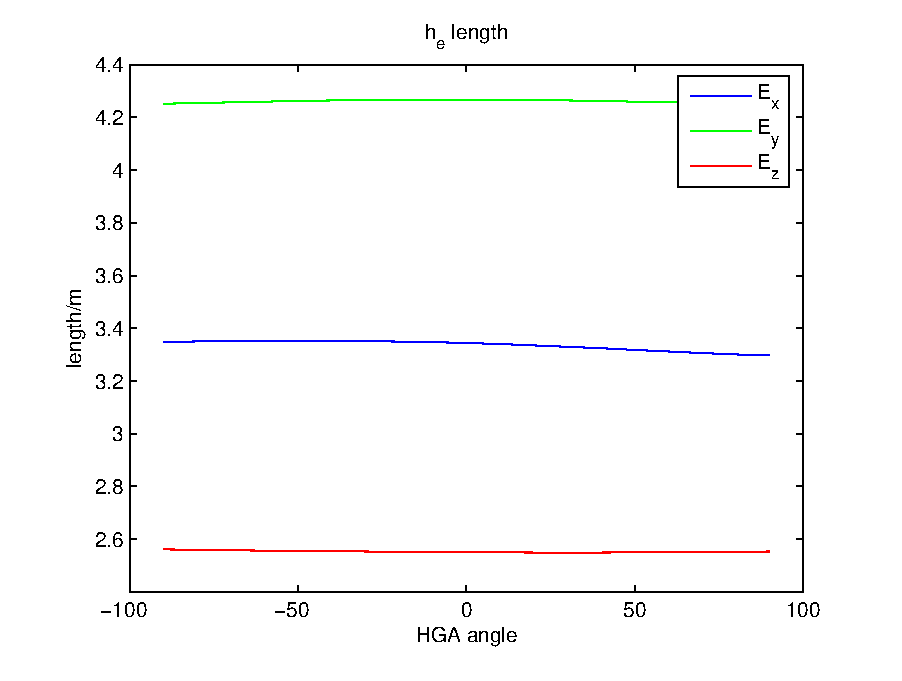
\includegraphics[width=7.6cm]{PaperPics/fig(13).eps}
\caption{\label{fig_var_HGA}Magnitude of the effective length vector as a function of HGA angle at 300kHz (left) and 10MHz (right)}
\end{figure}

\subsection{The impedances and capacitances}
Figure \ref{fig_imp_open} shows the antenna impedance for the STEREO antennas as a function of frequency. The imaginary part is plotted against the real part. At the frequency where the imaginary part is zero, the first resonance is located. At this frequency the impedance is purely resistive. The inclusion of the capacitances of the receiver, the cable, and the antenna mounting has the effect of decreasing the resonance frequency. In the case of transmitting antennas, the base capacitances are parallel to the antenna capacitances and both can be added and multiplied by $(\imath \omega)$ to yield the total admittance. To get the overall impedance matrix, the total admittance matrix has to be inverted. For details, see [\cite{macher07}].

\begin{figure}
\begin{center}
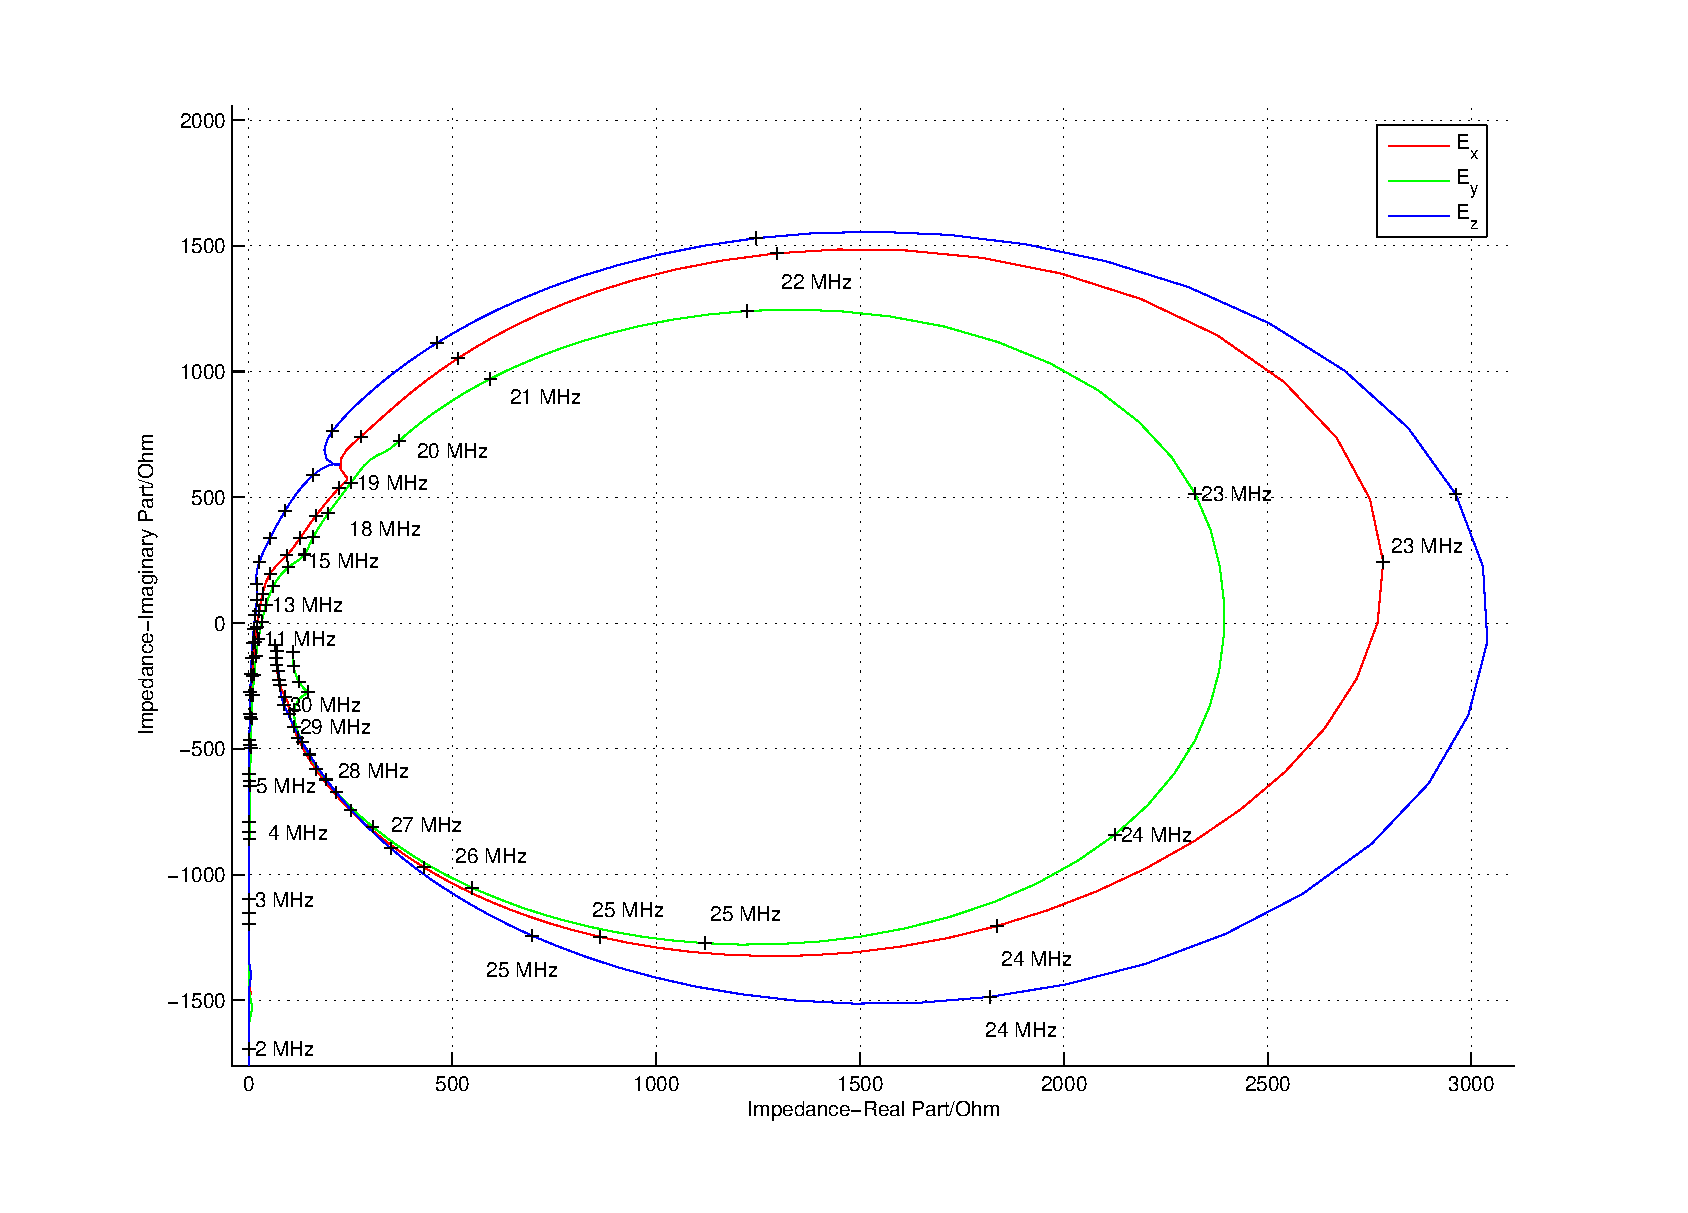
\includegraphics[width=12cm]{PaperPics/fig(14).eps}
\end{center}
\caption{\label{fig_imp_open}Real part vs. imaginary part of antenna impedance}
\end{figure}
%


\section{Conclusion}
In this paper numerical as well as experimental methods of spacecraft antenna calibration were described. Some results of these methods which were applied to the S/WAVES experiment on board the STEREO spacecraft were given for demonstration.

It is of vital importance that several methods are performed for each antenna system. Each method has its own advantages. Rheometry can be far more detailed than it would be possible for the wire-grid simulations, so the influence of the fine structure of the spacecraft can be estimated by comparison of the two methods. Therefore, rheometry is a good basis to decide about improvements of wire-grids, and yields a purely quasi-static result, which must agree with the asymptotic limit of the numeric calculations as the frequency converges to zero. The advantage of the computer simulation is the flexibility regarding the model structure, so it can be used to study the perturbation of antenna properties provoked by single spacecraft parts. Of course, the decisive advantage is that electromagnetic codes are devised for high-frequency analysis up to frequencies far above the resonance, thereby enabling the estimation of the validity range of the quasi-static results.

Figure \ref{fig_freq_range} compares the frequency ranges of the receivers of some spacecraft which where calibrated by using the mentioned methods. It is adapted from a figure published in [\cite{ruckerundi05}] The frequency ranges where the methods are valid are also depicted in the figure. Fortunately, the larger part of the frequency range of interest is at low or moderate frequencies where rheometry and the numerical methods are valid. Therefore, we can use both methods to complement and validate each other as was demonstrated in this paper.

An additional effect which has significant consequences for the behavior of STEREO's antennas is the influence of the surrounding space plasma. Currently research is performed on this topic and publications of its implication on the S/WAVES experiment are performed.


\begin{figure}
\begin{center}
\includegraphics[width=12cm]{PaperPics/fig(15).eps}
\end{center}
\caption{\label{fig_freq_range}Frequency ranges of radio experiments onboard certain spacecraft (red) together with the typical frequency ranges of the observed waves (dark red), and suitable antenna calibration methods.}
\end{figure}
%
\section{Acknowledgements}
The research leading to this paper was made possible by a project within the framework of the Austrian Space Applications Programme (ASAP-CO-001-05) of the Austrian Research Promotion Agency.

\begin{thebibliography}{24}

\harvarditem[Cecconi and Zarka]{Cecconi and Zarka}{2005}{cecconi05}
Cecconi, B. and P.~Zarka  (2005). Direction finding and antenna calibration
  through analytical inversion of radio measurements performed using a system
  of 2 or 3 electric dipole wire antennas on a 3 axes stabelized spacecraft.
  {\em Radio Sci.}{\bf 40}(3), doi:10.1029/2004RS003070.RS3003

\harvarditem[Collin and Zucker]{Collin and Zucker}{1969}{CollinZucker}
Collin, R.E. and F.J. Zucker  (1969). {\em Antenna Theory, Part 1}. McGraw-Hill
  Book Company Inc.

\harvarditem[Fischer {\em et al.}]{Fischer {\em et al.}}{2001}{cassini}
Fischer, G., W.~Macher, H.O. Rucker, H.P. Ladreiter and D.F. Vogl  (2001).
  Wire-grid modeling of cassini spacecraft for the determination of effective
  antenna length vectors of the rpws antennas. In: {\em Proc. Planetary Radio
  Emissions V} (H.O. Rucker, M.L. Kaiser and Y.~Leblanc, Eds.). pp.~347--356.
\newblock Austrian Academy of Sciences Press, Vienna.

\harvarditem[Fischer {\em et al.}]{Fischer {\em et al.}}{2003}{cassini2}
Fischer, G., W.~Macher, H.O. Rucker, H.P. Ladreiter and D.F. Vogl  (2003).
  Reception properties of the cassini/rpws antennas from 1 to 16 mhz. Poster at
  the EGS-AGU-EUG Joint Assembly, Nice.

\harvarditem[Harrington]{Harrington}{1968}{harrington}
Harrington, R.F.  (1968). {\em Field Computation by Moment Methods}. Robert E.
  Krieger Publishing Company.

\harvarditem[Macher]{Macher}{1997}{macher_dipl}
Macher, W.  (1997). Theorie effektiver Hoehenvektoren von Antennen mit
  Anwendung auf das radio and plasma wave science Experiment der Cassini
  Raumsonde. Master's thesis. University of Technology Graz.

\harvarditem[Macher {\em et al.}]{Macher {\em et al.}}{2002}{marsis}
Macher, W., B.~Schrausser, G.~Fischer, H.O. Rucker, H.~Lammer, C.~Kolb and
  G.~Kargl  (2002). Analysis of sounding antennas of the mars-express marsis
  experiment. In: {\em Proc. 2nd European Workshop on Exo/Astrobiology}
  (H.~Sawaya-Lacoste, Ed.). pp.~539--540.
\newblock ESA Publications Division, Noordwijk, ESA SP-518.

\harvarditem[Macher {\em et al.}]{Macher {\em et al.}}{2004}{marsis2}
Macher, W., H.O. Rucker, G.~Fischer and Marsis Team  (2004). Analysis of the
  marsis antenna system onboard mars express.
\newblock Poster at the EGU 1st General Assembly, Nice.

\harvarditem[Macher {\em et al.}]{Macher {\em et al.}}{2007}{macher07}
Macher, W., T.H. Oswald, G. Fischer, H.O. Rucker (2007). Rheometry of multi-port spaceborn antennas including mutual antenna capacitances and application to STEREO/WAVES.
\newblock Meas. Sci. Technol., 18, 3731-3742.

\harvarditem[Rucker {\em et al.}]{Rucker {\em et al.}}{2005}{ruckerundi05}
Rucker, H.O., W.~Macher, G.~Fischer, T.H. Oswald, J.-L. Bougeret, M.L. Kaiser
  and K.~Goetz  (2005). Analysis of spacecraft antenna systems: Implications
  for stereo/waves. {\em Adv. Space Res.} {\bf 36},~1530--1533.

\harvarditem[Rucker {\em et al.}]{Rucker {\em et al.}}{1996}{rheometry}
Rucker, H.O., W.~Macher, R.~Manning and H.P. Ladreiter  (1996). Cassini model
  rheometry. {\em Radio Sci.} {\bf 31}(6),~1299--1311.

\harvarditem[Sinclair]{Sinclair}{1950}{Sinclair}
Sinclair, G.  (1950). The transmission and reception of elliptically polarized
  waves. {\em Proc. IRE} {\bf 38},~148--151.

\harvarditem[Vogl {\em et al.}]{Vogl {\em et al.}}{2004}{vogl_04}
Vogl, D.F., B. Cecconi, W. Macher, P. Zarka, H.-P. Ladreiter, P. Fedou, A. Lecacheux, T. Averkamp, G. Fischer, H.O. Rucker, D. A. Gurnett, W. S. Kurth, and G.B. Hospodarsky (2004). In-flight calibration of the Cassini-Radio and Plasma Wave Science (RPWS) antenna system for direction-finding and polarization measurements.  {\em J. Geophys. Res. }
 {\bf 109}, doi:10.1029/2003JA010261.
\end{thebibliography}


\end{document}
